% !TEX program = tectonic
\documentclass[10pt,a4paper,twocolumn]{article}
\usepackage[margin=1.1cm]{geometry}
\usepackage[T1]{fontenc}
\usepackage[utf8]{inputenc}
\usepackage{lmodern}
\usepackage[french]{babel}
\usepackage{amsmath,amssymb}
\usepackage{booktabs,array,tabularx}
\usepackage{enumitem}
\usepackage{microtype}
\usepackage{graphicx}
\usepackage{xcolor}
\usepackage{titlesec}
\definecolor{bleu}{RGB}{20,45,90}
\definecolor{gris}{RGB}{90,90,90}
\definecolor{vert}{RGB}{0,110,60}
\definecolor{rouge}{RGB}{170,30,30}
\setlength{\columnsep}{0.55cm}
\setlength{\parindent}{0pt}
\setlength{\parskip}{2pt}
\setlist[itemize]{leftmargin=*,topsep=1pt,itemsep=1pt,parsep=0pt}
\titleformat{\section}{\normalsize\bfseries\color{bleu}}{}{0pt}{}[\vspace{-3pt}\titlerule]
\titlespacing*{\section}{0pt}{6pt}{3pt}
\begin{document}

\twocolumn[{\centering
{\LARGE\bfseries Résultat --- stratégie \og Calendar-Time Disclosure\fg{}\par}
\vspace{2pt}
{\small Notebook 08 $\cdot$ protocole pré-enregistré le 10/07/2026, exécuté d'un trait le même jour $\cdot$ verdict mécanique\par}
\vspace{6pt}}]

\section{Verdict : NO-GO --- pas d'alpha copiable, avec la puissance pour le voir}
Le test primaire S0 (achats d'actions divulgués, calendar-time, entrée J+1, fenêtre 21 j,
poids $\propto$ ADV$^{63}$ = réplication Pyun 2025, cap 10\,\%, rebalancement mensuel, 143 mois 2014--2026) :
\begin{center}\small
\begin{tabularx}{\linewidth}{@{}Xr@{}}
\toprule
$\alpha$ Carhart-4 \textbf{net} ($c=10$ bps/jambe) & $\mathbf{-0{,}77\,\%}$/an \\
$t$ (Newey-West 21 j) & $-0{,}48$ \\
$\alpha$ brut (avant coûts) & $+0{,}90\,\%$/an \\
Turnover (one-way, 2 jambes) & $16{,}5\times$/an \\
\textbf{Coût de break-even} & $c^{*}\approx\mathbf{5}$ \textbf{bps/jambe} \\
IR vs composite sectoriel & $0{,}01$ \\
$\beta$ Mkt / SMB / HML / MOM & \small$1{,}09$ / $0{,}02$ / $-0{,}12$ / $-0{,}04$ \\
DSR & $0{,}04$ \\
\bottomrule
\end{tabularx}
\end{center}
Aucun des 4 gates G2 pré-enregistrés n'est passé ($t\geq2$ ; $\alpha\geq150$ bps ; signe $>0$ sur les
2 moitiés --- obtenu : $-0{,}37\,\%$ pré-2020, $-1{,}09\,\%$ post-2020 ; IR sectoriel $\geq0{,}3$).
\textbf{Puissance} : $\hat\sigma_\varepsilon=1{,}67\,\%$/mois (procédure aveugle, cap maintenu à 10\,\%)
$\Rightarrow$ le test aurait détecté 35--47 bps/mois à 80\,\% --- l'effet revendiqué par la littérature
(50--90 bps) aurait été vu. \emph{Ce nul est une conclusion, pas une absence de test.}

\section{La grille fermée (12 tests) : 11 négatifs sur 12}
\begin{center}
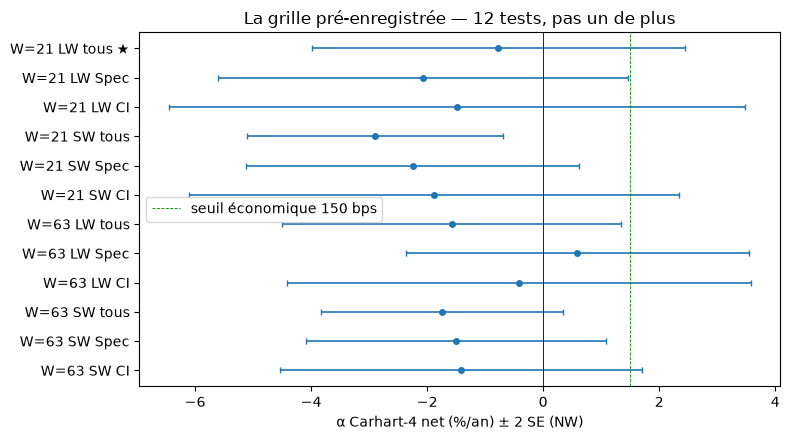
\includegraphics[width=\linewidth]{fig_08_forest.png}
\end{center}
Max $|t| = 2{,}63$ --- et c'est un $\alpha$ \textbf{négatif} : le portefeuille pondéré
$\log(1{+}\mathrm{NetBuy})$ (la \og conviction\fg{} des élus) fait $-2{,}90\,\%$/an. Avec l'équi-pondéré
(diagnostic) à $-3{,}06\,\%$/an ($t=-2{,}75$), on \textbf{réplique Chen-Sacerdote (2026)} : hors tilt
mégacaps, les achats du Congrès \emph{détruisent} de la valeur ; seule la pondération taille les ramène
vers zéro. Le bootstrap par blocs sur les 12 séries donne $q_{95}(\max t\,|\,H_0)=2{,}61$ : le 2,63 est
pile le bruit attendu (seuil de revendication : $t\geq3$). Les filtres de ma note (Spec, comité$\times$secteur)
n'aident pas ($t$ entre $-1{,}6$ et $+0{,}4$).

\section{La trace résiduelle --- et pourquoi elle est morte quand même}
L'event-study honnête (cohortes mensuelles, G1 descriptif) retrouve \emph{qualitativement}
Pyun/Lazzaretto : CAAR 21 j des achats \textbf{pondéré ADV} $=+49$ bps ($t=2{,}22$) vs SPY,
$+44$ bps ($t=2{,}68$) vs ETF sectoriel --- contre $-9$ bps en équi-pondéré. Le drift value-weighted
existe donc au niveau de l'\emph{événement}. Il ne devient pas un portefeuille rentable parce que :
\begin{itemize}
  \item une part du CAAR est du \textbf{bêta}, pas de l'alpha ($\beta=1{,}09$ : $\approx+0{,}8\,\%$/an
  reclassés par le modèle) et du multi-comptage des achats récurrents de mégacaps dans les cohortes ;
  \item le netting des ventes et l'agrégation par ticker diluent l'événement frais dans des positions
  quasi permanentes (top contributeurs : NVDA, AMZN, META, MSFT, AAPL) ;
  \item les \textbf{coûts} : à $16{,}5\times$/an, il faudrait exécuter sous $c^{*}\!\approx\!5$ bps/jambe ---
  sous les frottements réalistes, et sans compter le tax-drag du copieur.
\end{itemize}

\section{Contrôles et placebos (tous cohérents)}
\begin{itemize}
  \item \textbf{P1} dates décalées, \textbf{P2} tickers permutés, \textbf{P4} montants permutés
  ($B=1000$) : le $t$ observé est indistinguable du null ($p=0{,}61$ / $0{,}84$ / $0{,}66$).
  \item Ventes nettes $\approx0$ ($+0{,}59\,\%$, $t=0{,}35$) --- conforme à la littérature ;
  \item \texttt{owner=self} : $-3{,}37\,\%$/an ($t=-1{,}66$) --- les trades en compte propre ne sont pas meilleurs ;
  \item aucun membre ne porte seul le résultat (drop-one sur les 10 plus gros flux) ;
  \item ancrage du rebalancement ($+5/10/15$ j) : dispersion $\pm0{,}9\,\%$/an = bruit ; faillites : impact $\approx0$ bps ;
  \item capacité : poids $\propto$ ADV $\Rightarrow$ 100\,\% exécutable en 1 jour à 1\,\% de l'ADV jusqu'à 100 M\$ ---
  la stratégie était \emph{déployable}, elle n'est simplement pas rentable.
\end{itemize}

\section{Ce que ça ferme, ce que ça laisse ouvert}
\textbf{Fermé} : la dernière poche \og actions\fg{} réplicable de la littérature (drift post-disclosure
value-weighted) ne produit pas d'alpha net chez nous, avec le protocole le plus favorable
(grille pré-enregistrée, coûts réalistes à 10 bps, benchmarks multiples). Combiné aux notebooks 03--07
(copie par membre, top-K, secteurs, drift équi-pondéré), \textbf{le dossier \og copier les trades actions
du Congrès\fg{} est clos} : $\max t = 2{,}63$ sur 12 essais pré-comptés, $\mathbb{E}[\max t\,|\,H_0]=1{,}66$.
\par\textbf{Ouvert} (données nouvelles uniquement) : les \textbf{options} des PTR --- l'angle mort n\textsuperscript{o}\,1,
là où vivent la perf \og Pelosi\fg{} et les trades négatifs de Molk-Partnoy ; les jalons législatifs
(congress.gov) ; l'out-of-sample des mois à venir.

\vspace{4pt}
\hrule
\vspace{2pt}
{\footnotesize\color{gris} Protocole : \texttt{FICHE\_PREENREGISTREMENT\_08.pdf} (gelé avant exécution).
Détail complet, oracles de validation (moteur $<10^{-12}$, NW = statsmodels, équivalence 06) et figures :
\texttt{08\_Strategie\_Calendar\_Time.ipynb} (69 cellules, Run All 7 min hors téléchargements).}

\end{document}
